\documentclass[10pt,conference,compsocconf]{IEEEtran}

\usepackage{hyperref}
\usepackage{graphicx}	% For figure environment
\usepackage{color}
\usepackage{natbib}
\usepackage{float}
\usepackage{cprotect}
\usepackage{tabularx}
\usepackage{multirow}

\begin{document}
\title{Higgs Boson Challenge: Machine Learning Project}

\author{
  Robin Clerc, Pierre Vigier, Jacob Levy Abitbol\\
  \textit{Master of Computer Science, EPFL, Switzerland}
}

\maketitle

\begin{abstract}
  The CERN produces petabytes of data each day on the base of the ATLAS project, leading the research on the Higgs boson's decay.The often complex and high dimensional data sets generated in experiments are often hard to analyze and interpret. We give here an overview on how different learning methods perform on a collision event dataset.
  \end{abstract}

\section{Introduction}

The Higgs Boson is an elementary particle which explains why other particles have mass. It was discovered in collision experiments in the LHC, where proton bunches are accelerated on a circular trajectory in both directions. The collisions between the protons are detected by sensors of the ATLAS detector which also detect particles resulting from those collisions, resulting in the real-valued variables which we are provided with. These sensors however detect either actual interesting events or uninteresting events. The end goal of this project is then to improve the classification of the signal / background events, given the real-valued features resulting from the collision event.

\section{Models and Methods}
\label{sec:structure-paper}

\subsection{Data Exploration and Preprocessing}
The provided training dataset consists of a 250K samples corpus of collision events, where each event is classified as either signal $S$ or background $B$. Each collision is characterized by a set of 30 features from which the predictions will be made. A separate test set of unlabelled samples on which to test the performance of our models is also provided. \\
A first glance at our dataset reveals that overall,
more than 70\% of the events lack at least one feature, which is indicated in the data  by the value $-999$. These have to be imputed in order to be able to feed our dataset to a learning method. To handle this missing information we replaced the missing values of a given feature by its mean value, calculated separately for the training and the test set. \\
We also noticed that 15 \textcolor{red}{(Ce que moi j'ai mis. Apparemment vous en avez 12. A discuter) } out of the 30 available features included in the dataset seem to be power-law distributed. In order to compensate for the high skew of the observed distributions, we took the logarithm of these selected features instead of the actual features themselves (see Figure \ref{fig_kde}).\\ Each feature was then normalized using the means and standard deviations computed over the training set. 

\begin{figure}[htb]
\centering
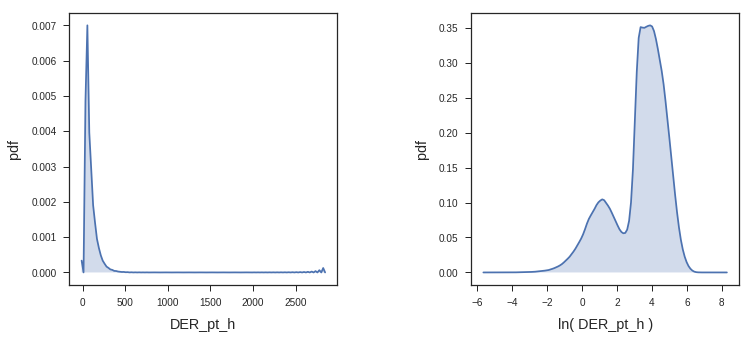
\includegraphics[width=\linewidth]{kdeplot.png}

\cprotect\caption{KDE plot for the modulus of the vector sum of the transverse momentum of the hadronic tau \verb+DER_pt_h+.
\emph{Left}: Original distribution. \emph{Right}:  Distribution of log values}
\label{fig_kde}
\end{figure}

%12 features take their values in a range describing several orders of magnitude in the positive values and with very sparse density in the high values.

The \verb+PRI_jet_num+ feature (a jet is a particle) is interesting because our correlation study highlights a very high correlations between features containing -999 values. Indeed -999 values are not actually features that sensors failed to catch, it is simply that they do not exist : if there is no jet, it has no speed, or if there is 1 jet we cannot compute any angle between jets. We can split those sets in 3 categories not having the same number of initial features.\\

\begin{figure}[H]
\centering
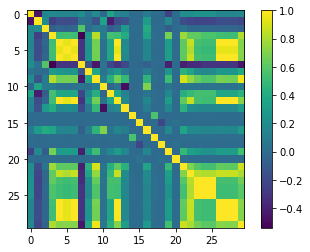
\includegraphics[width=\linewidth]{corr.png}

\cprotect\caption{Pairwise correlations of base features. Labels indicate the feature's index in the provided dataset. }
\label{fig_corr}
\end{figure}

We can see that the primitive features are highly correlated.

We also took notice that the \verb+PRI_jet_num+ feature, representing the number of particles or jets generated from the collision takes only 4 integer values (ranging from 0 to 3). This allowed to reduce the dimensionality of the original feature space by splitting our learning problem into 3 separate ones, each for a specific value of the number of jets (0,1,2-3).\\
This in turn enabled us to further remove static features from the dataset, yielding 19 features for  \verb+Jet 0+, 23 for \verb+Jet 1+ and 30 for \verb+Jet 2-3+ (see Table \ref{tab_feats})
\begin{table}[h!]
\centering
\caption{Missing values per feature and per jet value shown for features containing NaN (*: all, /: None)}
\footnotesize
\hspace{-0.2cm}
\begin{tabular}{ l| ccc } 
 \hline
   NaN Features & Jet 0 & Jet 1 & Jet 2-3 \\
 \hline
   \verb+DER_deltaeta_jet_jet+  & * & * & /  \\
   \verb+DER_lep_eta_centrality+  & * & / & / \\
   \verb+DER_mass_jet_jet+  & * & * & / \\
   \verb+DER_prodeta_jet_jet+  & * & * & /  \\ 
   \verb+PRI_jet_all_pt+  & * & * & /  \\
   \verb+PRI_jet_leading_eta+  & * & * & / \\
   \verb+PRI_jet_leading_phi+  & * & / & /   \\
   \verb+PRI_jet_leading_pt+  & * & / & / \\
   \verb+PRI_jet_subleading_eta+  & * & / & / \\
   \verb+PRI_jet_subleading_phi+  & * & * & /  \\
   \verb+PRI_jet_subleading_pt+  & * & * & /  \\
  \hline
\label{tab_feats}
\end{tabular}
\end{table}

Finally, the difference of the particle azimuthal angles $\Phi$, namely, \verb+PRI_tau_phi+, \verb+PRI_lep_phi+, \verb+PRI_met_phi+, were considered to be of potential interest  in determining the nature of the collision detected and were therefore added as features.

Then, depending on the result of the grid search on the different methods and jets, we add a certain number $n$ of polynomial features from each initial feature. And then we build the cross terms of the base features, and add their $\sqrt{n}$ first polynomial features. Thus when the degree $n$ of the base features improves we still keep a descent proportion of cross terms.

\subsection{Different methods tested}

For each of the following algorithms we performed either a 4 or a 10 fold cross validation for each element in the grid search to check the robustness of our models.

We made the choice to use the different methods following their number of meta parameters to keep an order of magnitude of the performances.

\subsubsection{Least squares}

In this method we just have to chose the degree of the polynomial features. This method was very efficient without cross terms but when we added the cross terms (and solve the problem of the singular matrix thanks to a gradient descent or the pseudoinverse) we got worse performances that we interpreted as over-fitting ; it was time to switch to a more complex model to counter it thanks to a penalization.


\textcolor{red}{A enlever : Our first submissions were made thanks to this algorithm, but when we added cross terms we had to use the gradient descent version as the matrix became singular Il y a une facon de resoudre ca en passant par la decomposition en SVD et la pseudoinverse. After a grid search to find the best degree, we decided to add a new parameter and thus perform a Ridge regression to avoid over-fitting. }

\subsubsection{Ridge regression}

Once again, we performed a grid search to know what were the best degree and the best $\lambda$ to use.

As expected, it was not the same for the 3 sub categories. We got :
\begin{table}[h!]
\centering
\caption{Results of the grid search with cross terms \%)}
\footnotesize
\hspace{-0.2cm}
\begin{tabular}{ l| ccc } 
 \hline
   Jet & Degree & Lambda & 10-fold Accuracy  \\
 \hline
   \verb+Jet 0+  & 11 & $10^{-15}$  & 0.845941347212  \\
   \verb+Jet 1+  & 12 & $10^{-15}$  & 0.802476141346 \\
   \verb+Jet 2-3+  & 14  &  $10^{-13}$ & 0.826619795975 \\
  \hline
\label{grid_search_ridge_cross}
\end{tabular}
\end{table}


As shown, in Table \ref{tab_first_run}, the use of the  more sophisticated Newton based  gradient descent methods was hindered by the the non-invertible nature of the Hessian matrix. Instead of implementing quasi-Newton methods to work around this condition, we chose to focus on the three first models. Also, the gradient descent using the SGD variant with a batch size of 33\% of the training samples due to the high number of samples and features that were studied jointly. 
 
\begin{table}[h!]
\centering
\caption{Initial training results (Model predictive accuracy \%)}
\footnotesize
\hspace{-0.2cm}
\begin{tabular}{ l| ccc } 
 \hline
   Model & Jet 0 & Jet 1 & Jet 2-3  \\
 \hline
   \verb+linear_regr+  & 82.56 &74.18  & 77.68  \\
   \verb+ridge_regr+  & 82.50 & 74.17  & 77.67 \\
   \verb+log_regr_gd+  & 83.03  &  76.82 & 81.27 \\
   \verb+penal_log_regr_gd+  & * & * &  * \\ 
   \verb+log_regr_newton+  & / & / & / \\
   \verb+penal_log_regr_newton+ &  / & / & / \\
  \hline
\label{tab_first_run}
\end{tabular}
\end{table}




\end{document}
\subsection{Data preprocessing}

As previously stated, we split the sets in 3 categories:  
\begin{itemize}
    \item $Jet0$ for which we exclude the 12 constant features
    \item $Jet1$ for which we exclude the 8 constant features
    \item $Jet{2;3}$ 
\end{itemize}

We log-transform the features taking their values in several orders of magnitude.

The we standardize each category by :
\begin{itemize}
    \item Getting the mean and the standard deviation of the training set category.
    \item Normalize the training set category
    \item Normalize the test set category with the mean and standard deviation of the training set.
\end{itemize}

\subsection{Feature engineering}

 First of all, as we are provided with angles, it can be interesting to add as a feature the absolute differences between those angles to extract more information.








